This chapter lays out the implementation by presenting an architectural overview on how and where the proposal can be included in the Graal.js project which is further detailed in the upcoming sections. The implementation explanation is then wrapped up by explaining the interaction with dynamic imports and the serialization / deserialization framework.

\section{General overview}
Before thinking about implementing the proposal into the Graal.js project one needs to know how source code is evaluated by Graal.js. The path of source code going through the project is straightforward. Without going too deep into the specifics it follows figure \ref{fig:mainImpl}. The source code is traversed and transformed into a token stream. This token stream is then evaluated by the parser which uses the found token in conjunction with the specified grammar given by ECMAScript \cite{ecma} to transform the token into an intermediate tree form. This tree contains nodes representing general language concepts without specifying the nodes into specialized forms. As can be seen in Figure \ref{fig:mainImpl} a module block is represented by a function node in the intermediate form. Later on in the translation pipeline the \texttt{GraalJSTranslator} class is called with an intermediate form node and translates it into a specialized form. In the scope of this thesis a \texttt{FunctionNode} to a \texttt{ModuleBlockNode}. These specialized nodes are then executed when being visited in the tree. On the specifics of interpretation and compilation during execution see Section \ref{sec:graalcomp}. 

\begin{figure}[h!]
    \centering
    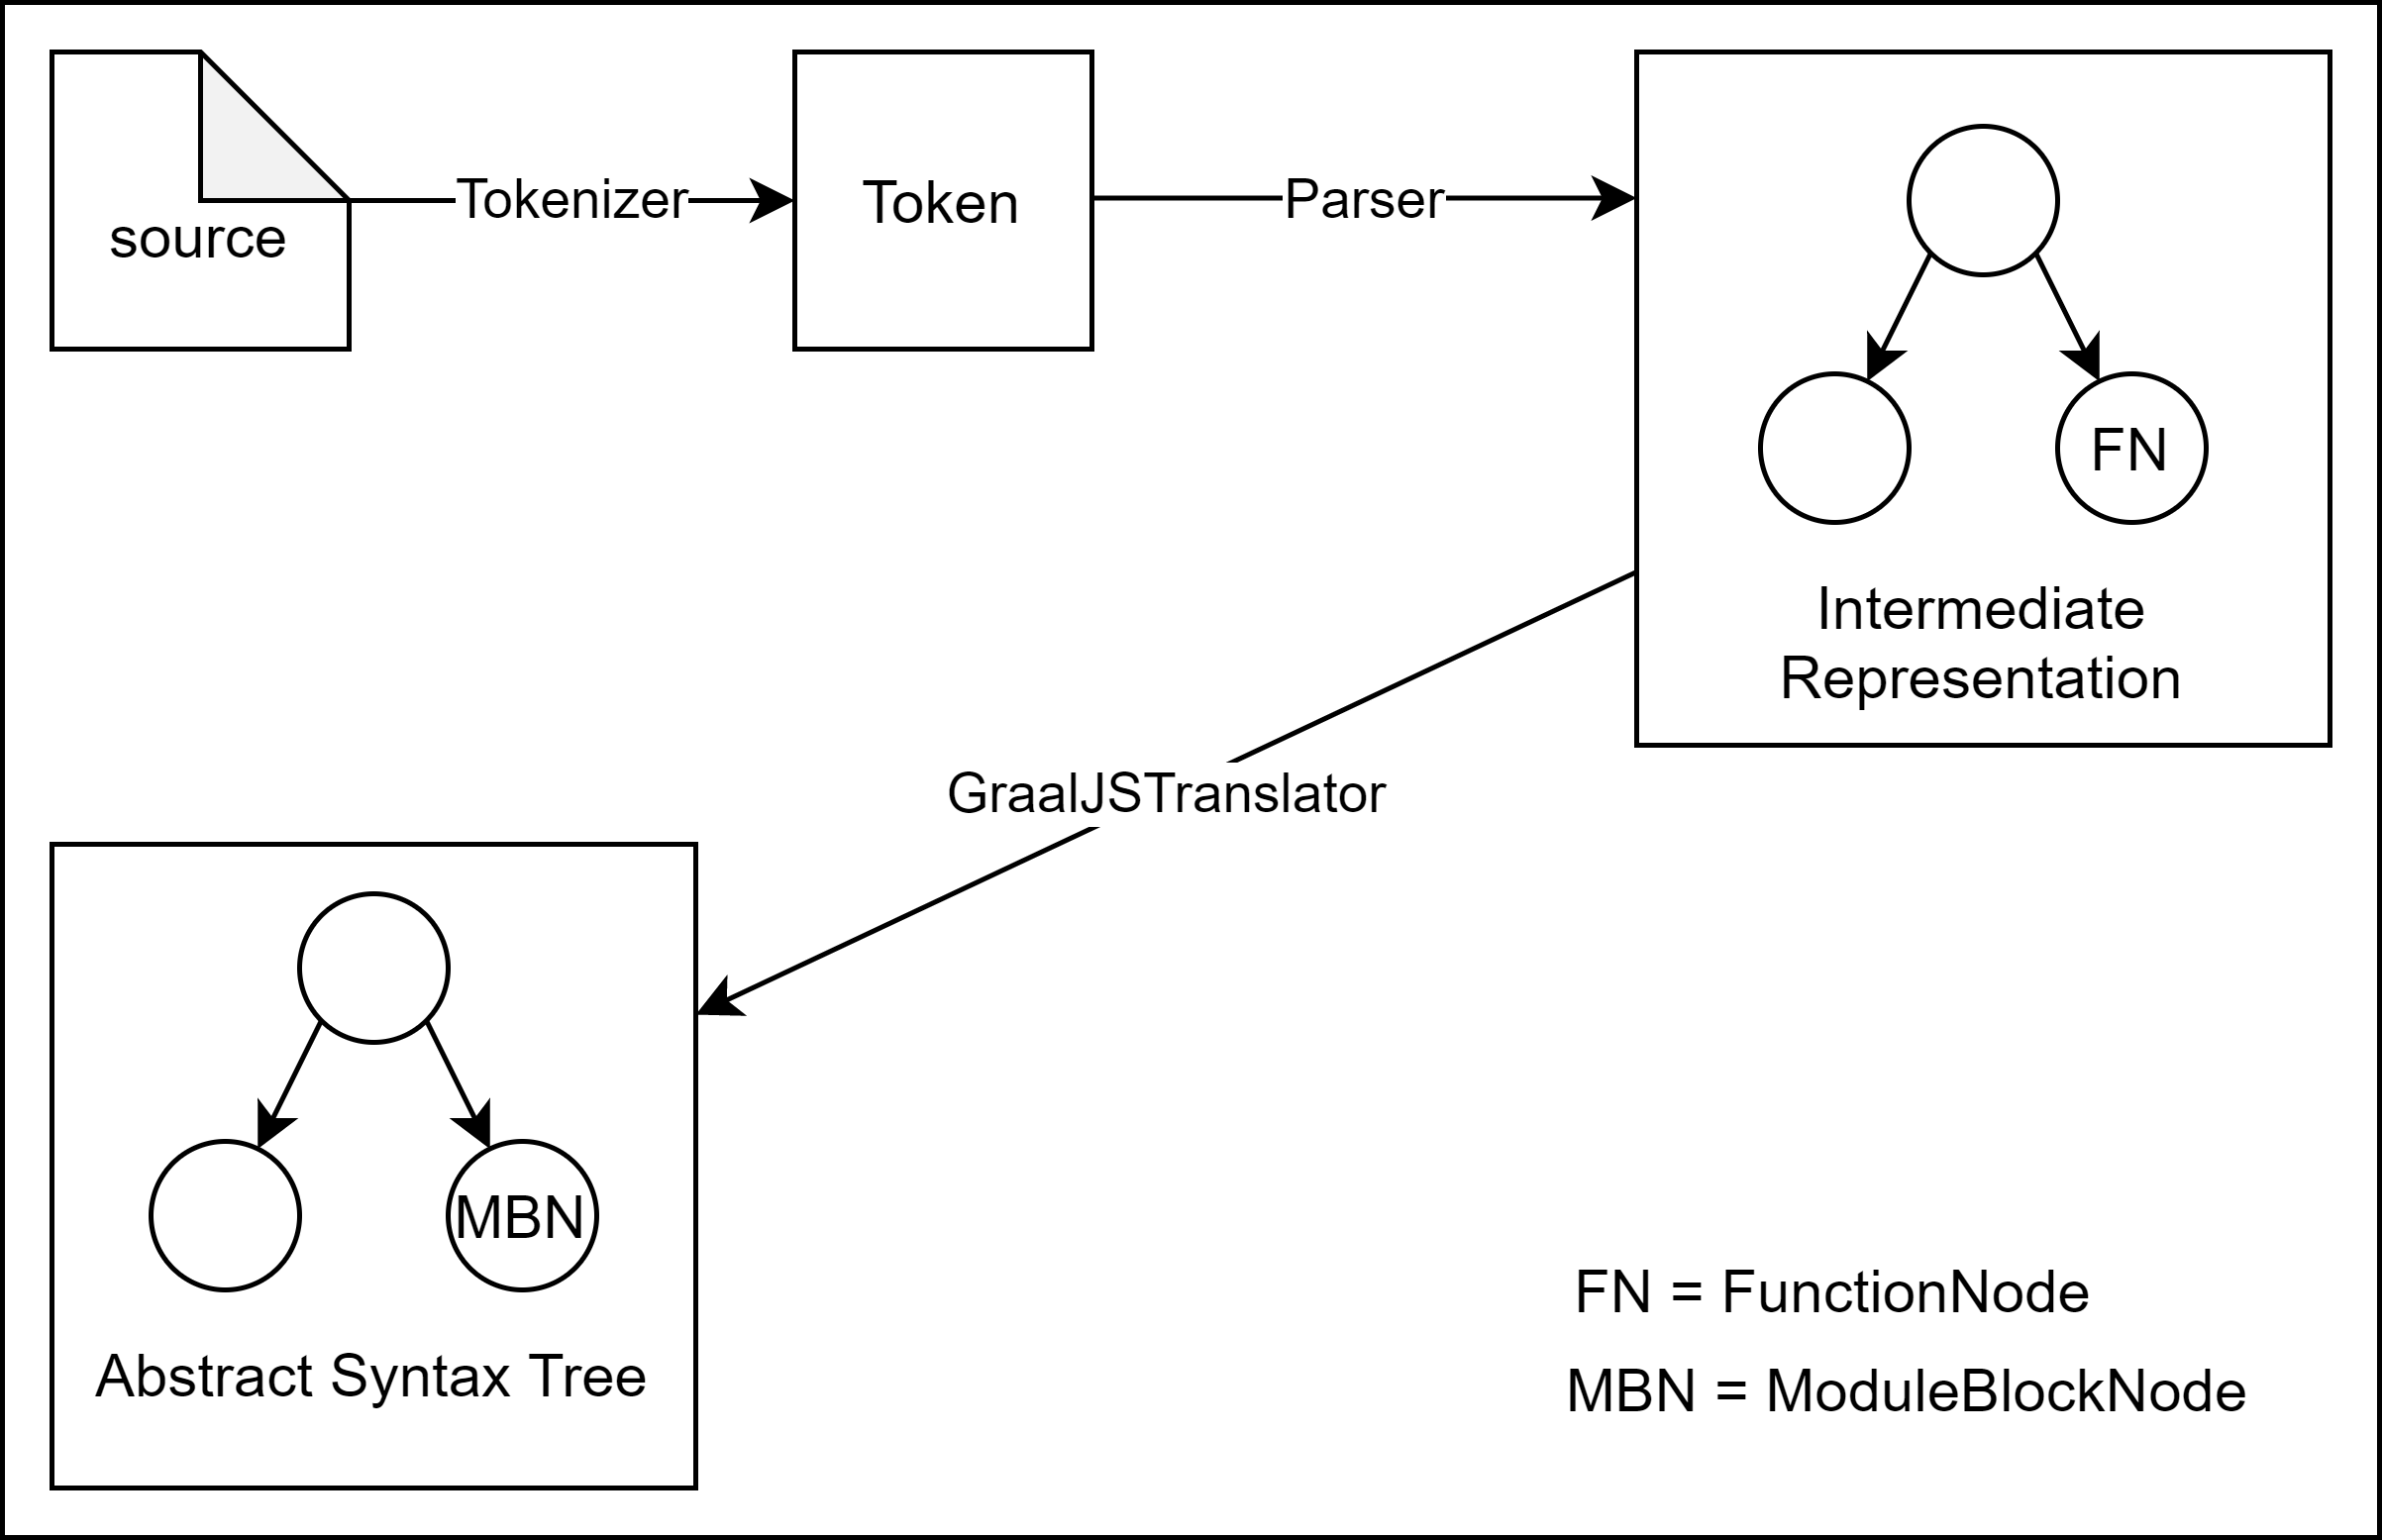
\includegraphics[scale=0.165]{figures/implMain.png}
    \caption{Code evaluation by Graal.js}
    \label{fig:mainImpl}
\end{figure}

Implementing the module block proposal into the Graal.js project involves several steps. Those are adjustments to the parser to capture the newly introduced syntax, implementation of the prototype, introducing a new respective node for module blocks and lastly adjusting the node for dynamic import-calls. At this point the implementation is limited to the available specification of the proposal. The chapter's outline is firstly the module block direct implementation into the Graal.js project followed by explanations of some necessary adjustments for dynamic import-calls. The direct implementation part is split up in four parts: parser changes, module block node, constructor and the prototype.The specific parser changes are explained in the next section.

\section{Parser}
From the specification we can take away that \texttt{module} won't be introduced as a keyword in ECMAScript meaning during parsing the word will be treated as an identifier. As both, identifier and module blocks, are classified as so called \texttt{PrimaryExpressions} the main change is happening in this explicit parser method inplace of the "ident"-Token branch. Like Listing \ref{lst:impl:minModule} shows \texttt{module} can still be used as identifier. Thus recognizing a module block needs a lookahead token and additionally satisfy the no line delimiter condition. This is done by first checking for the next token being a \texttt{\{} after a \texttt{module} identifier , changing from the "ident"-branch to the module block branch and then checking whether there is at least one line delimiter between the \texttt{module} and the \texttt{\{}. A line delimiter occurrence would result in a syntax error. Otherwise the parsing continues with capturing all statements inside the module block similar to a regular module and then putting the result into the same intermediate representation form a regular module would be put in. This caters to the notion of modules and module blocks acting similar in the language specification. The only relevant difference is the end of the parsing which is the end of file in the module case and a closing brace (\texttt{\}}) in the module block case. The next section talks about further steps that are taken during translation.

\begin{lstlisting}[caption={Minimal module identifier example in JavaScript}, label={lst:impl:minModule}]
    var module = 42;
    
    var moduleBlock = module { };
\end{lstlisting}

\section{ModuleBlockNode: Module Blocks' Truffle AST representative}

The Graal.js project includes a class called \texttt{GraalJsTranslator}. This class is generally speaking for translating the intermediate representation nodes into specialized ones for the resulting AST. During execution of this class the intermediate module block representative gets translated into a module block node. The node is built according to the provisional proposal's specification meaning the hidden properties are set as defined. At the current point the \texttt{hostInitializeModuleBlock}-method which is mentioned in the specification is not implemented as it is not included in the specification yet. With the node representation itself finished the next section turns towards the prototype and the constructor.

\section{ModuleBlock prototype and constructor}

This part of the implementation is split up into two parts where firstly a discussion is depicted as to why the constructor is specified as is. Secondly the actual implementation is explained. At current state, as of July 2021, it is unwished for by the developers to implement yet another eval-esque structure coming from the desire for less dynamic evaluation. A point for including an actual constructor for module blocks would be the symmetry and consistency in the whole language's specification. This concern can be brought up since structures like \texttt{AsyncFunction} or \texttt{GeneratorFunction} do have constructors with a code-string parameter. Right now the eval-point outweighs the symmetry-/consistency-point. The constructor when called simply throws a type error. This concludes the rather simple implementation of the constructor with the discussion behind it maybe resulting in a change of the constructor's specification. The next paragraph concludes the implementation of the module block itself by introducing the module block prototype.

The prototype is fairly simple constructed. Its prototype property is the module block Prototype Object with the general attributes writable, enumerable and configurable all set to false as is standard in the ECMAScript specification. The module block Prototype Object is \texttt{\%ModuleBlock.prototype\%}. Its internal prototype slot is \texttt{\% Object.prototype \%} and it is an ordinary Object. It has simply one function which is the toString() method. This method should check whether it is used on a \texttt{ModuleBlock} object and as such return the hidden \texttt{SourceText} property.
On a second note \texttt{ModuleBlock} is specified as global. This allows for \ref{lst:impl:globModule} to work. Again this matter can be subject to change during the proposal's progress.

 \begin{lstlisting}[caption="ModuleBlock working as global in JavaScript", label="lst:impl:globModule"]
        var moduleBlock = module { };
        
        moduleBlock instanceof ModuleBlock; // true
\end{lstlisting}

This concludes the module block implementation itself. The module block's syntax is implemented in the parser, the module blocks runtime semantics are implemented in the specified module block node for the resulting AST and the constructor's and prototype's specification is met accordingly with also registering ModuleBlock as global. In conclusion the module block at this state is implemented as a standalone without much interaction with the rest of the EcmaScript ecosystem. This leads us to the question how does the module block interact with existing language features. The proposal's specification only states one interaction with another language feature: the import()-call. Thus the next paragraph states the necessary changes for integrating module blocks into the dynamic import calls.

\section{Interaction with dynamic import}

Hence, only the Graal.js representative, the class ImportCallNode, needs to be changed in this matter. The main difference is the change from using only Strings with the module's URL as identifiers to using the module block node as identifier for the resulting Module Record. To accomplish this, the object needs to be checked and if it does not satisfy the condition of being an object with the internal slot of ModuleBlockBody, a String is then used as identifier, otherwise the ModuleBlockNode. After that the regular HostImportModuleDynamically routine is called as would be for regular modules. This results in a Module Record which is saved in the module map. The module map itself also has to be changed to accept the module block node as key as well as the URLs used for regular modules. During that process the three-step phase of modules is executed. First the ModuleBlock source code gets parsed as it would be a separate module. It is then instantiated and at last evaluated. Through these explicit inner workings the module block preserves the positive effects of modules while eliminating the aforementioned negatives.\\

The state at July 2021 the dynamic import is the only interaction being inflicted by the module block proposal. With the changes made on the ImportCallNode and the aforementioned changes to the parser, the introduction of the ModuleBlockNode and the registration of the respective prototype and constructor the implementation phase is finished. As already mentioned some specifics might have to be changed in the future as the proposal matures through the stages but the skeleton is led out at this state. The following paragraph and figure \ref{fig:blockVSmodule} conclude the implementation on a comparison between modules and module blocks on implementation level behavior.

\section{Serialization framework}

This section presents the framework for transferring module block source code from one process to another, i.e. one machine to another. For this to be possible two functions have to be implemented and registered at the global object in JavaScript. Their names exactly match their purpose: \texttt{serialize} and \texttt{deserialize}. The serialize method is straightforward and is oriented on the \texttt{toString}-method by accessing the \texttt{SourceText} property and then taking the string gained from the access and turning it into a byte-array. Fortunately, Java itself has a builtin method for strings turning them into a byte array using the executing platform's standard charset. This already concludes the serialization of a module block. The deserialization involves a few more steps. The given byte-array has to be turned back into a string, which again is builtin into Java, as the string class has a constructor taking a byte-array and a charset. Then an internal source object has to be created. The source object is created via the beforehand created string. Then the source code has to be parsed and translated as explained in Sections 3.2 and 3.3.

\section{Wrap up}

On regard of parsing the main difference between module blocks and modules is the outside call onto the class when parsing modules but module blocks have to be caught from inside the parser. Hence the parser is told explicitly to parse a module from another class while a module block is caught by the inner class's logic and will from then on be treated similarly to the regular module. Both parsing results are then encapsulated into the same intermediate representation as a \texttt{FunctionNode}. When translating this intermediate representation into the final AST representative the path of modules and module blocks splits up again as the module block is transformed into a \texttt{ModuleBlockNode} and the module is transformed into a \texttt{JSFunctionExpressionNode}. Finally as those constructs are imported, in the module's case also statically, dynamically the final result will always be a \texttt{JSModuleRecord} which is the AST's representation of the, in ECMAScript specified \cite{ecma}, Module Records. The description is also envisioned by the subsequent figure \ref{fig:blockVSmodule} This brief difference in behavior explanation concludes the implementation chapter which is followed by the evaluation chapter detailing the testing of the as set out above implementation.

\begin{figure}[h!]
    \centering
    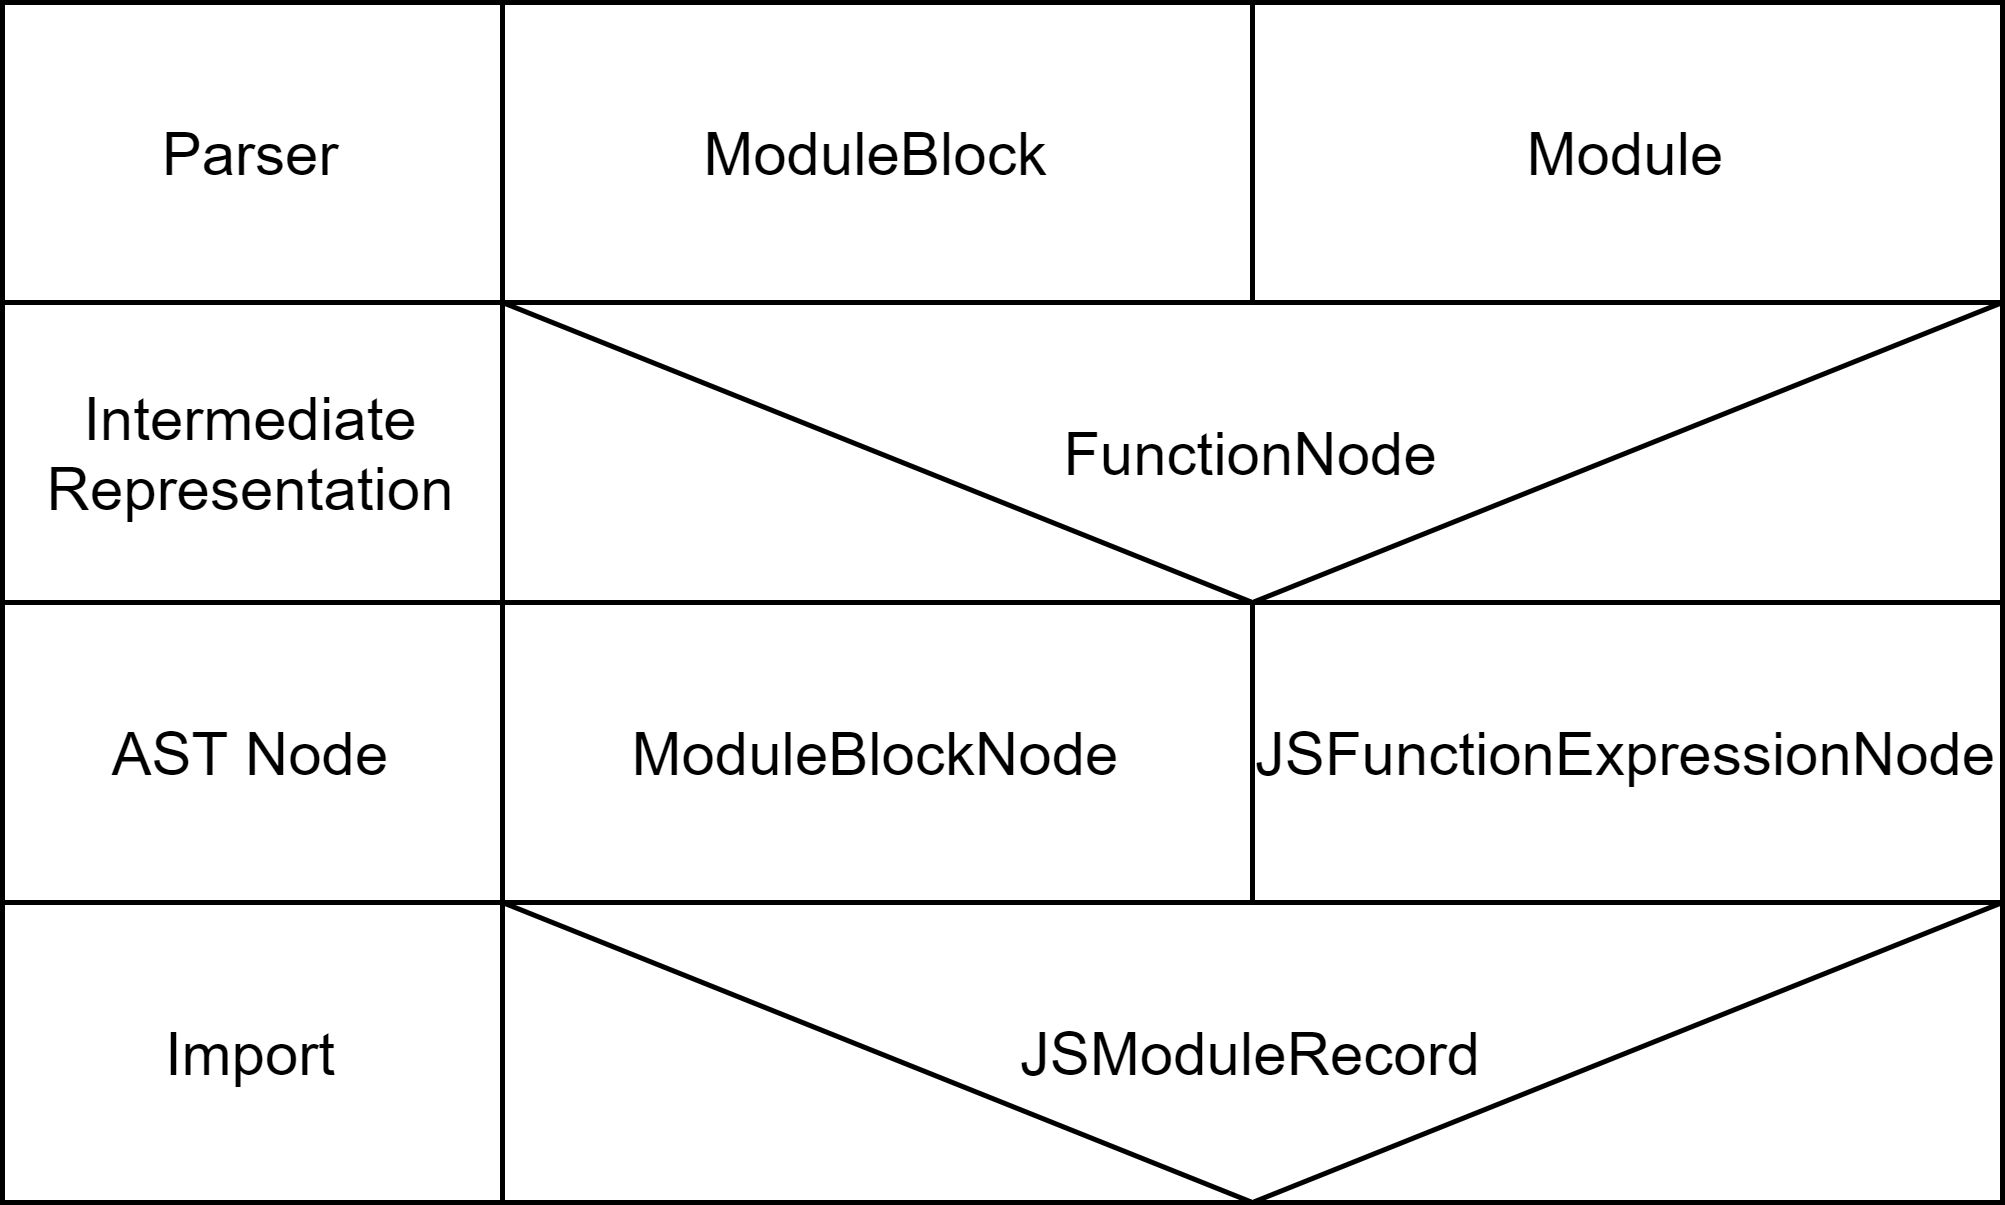
\includegraphics[scale=0.165]{figures/ModuleBlockVSModule.png}
    \caption{Simplified GraalJS translation pipeline of module blocks and modules}
    \label{fig:blockVSmodule}
\end{figure}